% !TEX root = thesis.tex
{
\cleardoublepage% Move to first page of new chapter
\let\cleardoublepage\relax% Don't allow page break
\noindent \small{Based on: \emph{Probabilistic modelling of general noisy multi-manifold data sets}, Canducci~M., Ti\v{n}o~P., Mastropietro~M. Submitted to \emph{Artificial Intelligence} \citet{Canducci2021}.
This work has been carried out during the planned SUNDIAL secondment at the Computer Science Department of the University of Birmingham.
}
\chapter{Low-dimensional manifolds}
\label{ch:manifolds}
}

\abstract{
The intrinsic nature of noisy and complex data sets is often concealed in low-dimensional structures embedded in a higher dimensional space.
%Number of methodologies have been developed to extract and represent such structures in the form of manifolds (i.e. geometric structures that locally resemble continuously deformable intervals of $\mathbb{R}^j$ \footnote{$j$ is the manifold dimensionality.
%Mathematically, continuous deformation corresponds to homehomorphism: one-to-one continuous mapping with continuous inverse.}).
% Usually a-priori knowledge of the manifold's intrinsic dimensionality is required.
% Additionally, their performance can often be hampered by the presence of a significant high-dimensional noise aligned along the low-dimensional core manifold. 
In real-world applications, the data can contain several low-dimensional structures of different dimensionalities.
We propose a framework for dimensionality estimation and reconstruction of multiple noisy manifolds embedded in a noisy environment.
To the best of our knowledge, this work represents the first attempt at detection and modelling
of a set of coexisting general noisy manifolds by uniting two aspects of multi-manifold learning: 
the recovery and approximation of core noiseless manifolds and the construction of their probabilistic models.
The easy-to-understand hyper-parameters can be manipulated to obtain an emerging picture of the multi-manifold structure of the data.
% We demonstrate the workings of the framework on two synthetic data sets, presenting challenging features for state-of-the-art techniques in Multi-Manifold learning.
% The first data set consists of multiple sampled noisy manifolds of different intrinsic dimensionalities, such as M\"{o}bius strip, toroid and spiral arm. The second one is a topologically complex set of three interlocked toroids. 
% Given the absence of such unified methodologies in the literature, the comparison with existing techniques is organized along the two separate aspects of our approach mentioned above, namely manifold approximation and probabilistic modelling. 
The framework is then applied to a complex data set containing simulated gas volume particles from a particle simulation of a dwarf galaxy interacting with its host galaxy cluster.
Detailed analysis of the recovered 1D and 2D manifolds can help us to understand the nature of Star Formation in such complex systems.
}
\section{Introduction}


Dimensionality reduction and Density Estimation of raw data, are commonly used tools to extract information from complex and noisy data sets.
Due to dependencies among measured attributes of real world data,
the data is often distributed along low-dimensional structures in a higher dimensional measurement space.
This realisation has driven the development of a variety of Manifold Learning algorithms.
Principal Component Analysis \citep[PCA, ][]{Pearson1901} is a well understood and widely used linear dimensionality reduction scheme. 
%\Marco{It can be considered the progenitor of Manifold Learning, where the data is assumed to lie on a multivariate Gaussian and the recovered principal components capture the variance of the data along orthogonal directions.}
However, by design, PCA cannot appropriately capture non-linear low-dimensional structures.
% This lack of flexibility has been addressed by non-linear dimensionality reduction algorithms such as Isomap \cite{Tenenbaum2319}
% and Locally Linear Embedding \citep[LLE][]{Roweis00nonlineardimensionality},
% where the manifold is approximated by a neighbourhood graph and a neighbouring preserving map respectively.
% Both methods take advantage of the definition of a manifold as a locally linear low dimensional structure of dimension $j$.

% Many other Manifold Learning algorithms aiming to provide suitable approximations to low-dimensional data manifold have been proposed.
% Examples include Laplacian eigenmaps \citep{Belkin01laplacianeigenmaps},
% Hessian eigenmaps \citep{Donoho5591},
% Local Space Tangent Alignment \citep[LSTA, ][]{Zhang02principalmanifolds},
% C-Isomap \citep[an extension of Isomap to conformal embeddings][]{Silva:2002:GVL:2968618.2968708},
% NMDS \citep[non-metric formulation of Multidimensional Scaling (MDS)][]{doi:10.1002/bs.3830040308, Cox2008, Kruskal1964},
% Riemannian Manifold Learning \citep[RML, ][]{10.1109/TPAMI.2007.70735}.

% In \cite{boissonnat:hal-01615863} (and bibliographic references therein) a different angle, based on computational geometry, 
% has been proposed in order to extract low-dimensional manifolds from data samples.
% Here, simplicial complexes (such as Delaunay triangulations, $\alpha$-complexes and filtrations)
% are used for manifold reconstruction.
% With these techniques it is possible to infer geometrical and topological properties of data points 
% that uniformly sample a single manifold embedded in a higher dimensional space.

% While such techniques are potentially powerful and theoretically well grounded,
% their capability to naturally handle high-dimensional noise aligned along low-dimensional manifolds is limited.
% Besides the sensitivity to the noise issues, it is often required that the intrinsic data dimensionality is known a priori. 

Generative Topographic Mapping \cite[GTM, ][]{Bishop1998GTMTG} was proposed as a probabilistic formulation of the Self-Organizing Map \citep{Kohonen1982}.
Its main advantage is that instead of treating noisy manifold as a core low-dimensional manifold to be discovered,
plus some ``noise" around it that somehow needs to be dealt with, 
it formulates a consistent manifold-aligned density model in the form of a constrained mixture of Gaussians.
The location parameters (means) of the Gaussian components are constrained to lie on a smooth manifold 
-- most commonly a smooth image in the data space of a two-dimensional interval (latent space). 
The original GTM formulation is trained in the maximum likelihood framework using the the Expectation-Maximization (E-M) algorithm \citep{10.2307/2984875}.
Because of the sensitivity to initialization, a suitable initialization is required (e.g, using PCA).
% Bayesian formulations of GTM have also been proposed \cite{Olier2008VariationalBG}.

Other global density estimators, whether non-parametric, e.g. Parzen windows \cite{parzen1962estimation}
(and its extensions such as Manifold Parzen Windows \cite{NIPS2002_2203}, Fast-Parzen Windows \cite{5178637}),
or semi-parametric, e.g. Infinite Gaussian Mixture model\cite{10.5555/3009657.3009736},
are not designed to extract a representation of the embedded low-dimensional structures.
They also may be computationally expensive to train and/or evaluate. 

% To deal with complex data sets, where several manifolds of different dimensionalities can co-exist,
% generalizations of the previous methods have been developed:
% Multi-Manifold Discriminant Analysis (MMDA, \cite{Yang:2011:MDA:1963661.1963809}),
% Sparse-Manifold Clustering and Embedding (SMCE,\cite{NIPS2011_4246}),
% Multi-Manifold Isomap (M-ISOMAP\cite{Fan2012IsometricML}),
% Multi-manifold Proximity Embedding  (MPE,\cite{Fan:2016:EIM:2903049.2903101}),
% Multi-Manifold LLE (MM-LLE,\cite{Hettiarachchi:2015:MLL:2791619.2792198}),
% S-Isomap++ \cite{2017arXiv171006462M},
% Hierarchical GTM \cite{Tino_PAMI_2002}.
% However, based on the same assumptions as their predecessors, the methods still need to be informed
% about the dimensionalities of the different manifolds 
% and struggle when dealing with topologically complex, noisy structures}.

In \citet{Canducci2021} we propose a framework for automated dimensionality estimation and reconstruction 
of multiple noisy manifolds embedded in a noisy environment.
We generalize the GTM model so that densities aligned along arbitrary manifolds
(even non-orientable ones - such as M\"{o}bius strip) can be captured.
This is achieved by replacing the simple Euclidean latent space (generally parametrized as a discretized interval of $\mathbb{R}^j$)
with an abstract graph reflecting the topology of the data manifold that, when embedded in the data space,
provides a manifold skeleton around which the noise models can be organized.

The work is inspired by \cite{10.1007/978-3-540-87481-2_37}, but extends and generalizes it threefold: 
\begin{itemize}
 \item it proposes a new robust dimensionality index estimation for data points,
 \item through a dedicated manifold crawling mechanism it allows for completely abstract manifold representations in the GTM latent space (instead of a regular grid), and
 \item it has Gaussian noise components naturally aligned along the manifold, unlike the spherical noise models in the original GTM and \cite{10.1007/978-3-540-87481-2_37}.
\end{itemize}
Manifold aligned noise models in GTM were also considered in \cite{Bishop1998DevelopmentsOT},
but under the assumption of simple latent space structure in the form of $j$-dimensional interval.
The key idea was to impose larger and smaller variances in directions locally parallel and perpendicular, respectively, to the manifold.
Since our latent space is a discrete structure (abstract graph representing a skeleton of a given manifold),
we formulate local noise models through kernel based estimates of the local covariance matrix of the data,
with trainable scale parameter to allow for optimized overlapping of the neighbouring Gaussian components. 

Our work presents a radical reformulation of GTM to capture and model low-dimensional general noisy manifolds
through a dedicated abstract graph-structured latent space reflecting the core manifold structure, specific to each noisy manifold.
% \citet{Bacciu13} present another radical generalization of GTM in the reverse direction -
% this time keeping the original simple latent space structure, but allowing for abstract structure in the data space - the space of trees.

The paper has the following organization: in section \ref{sec:Methodology} we set up the scene,
explain the broad outline of the methodology and introduce the synthetic data set on which different steps of the methodology will be demonstrated.
Section \ref{sec:AGTM} introduces the core model of our methodology, Abstract GTM (AGTM),
representing density aligned along a single manifold.
We explain how the abstract latent space graph representing topology of the data manifold is
extracted through manifold crawling and how this graph is then embedded in the data space along with the suitable set of noise models.
We also show how to calculate local curvature at the edges of the embedded graph,
taking advantage of the smooth manifold description provided by AGTM.
Section \ref{sec:MultiManifold} defines our notion of Dimensionality index for individual points
and extends the framework of section \ref{sec:AGTM} to the multi-manifold case.
We also offer a computationally efficient alternative to Multi-Manifold Crawling.
The price to pay for gains in efficiency is weaker detection stability of low dimensional manifold entities buried in the data.
% Section \ref{sec:Comparison} presents an experimental comparison on two synthetic data sets of our methodology
% with alternative multi-manifold learning and probabilistic modelling methods.
Even though our methodology aims to provide density models of multiple low-dimensional manifolds buried in the data,
we organise the comparative experiments separately for the multi-manifold capture and probabilistic modelling aspects of our work.
This is because to the best of our knowledge, no other method exists that can simultaneously recover low dimensional
representations of an unknown number of manifolds while building their probabilistic models.

Our main contributions can be summarized as follows:
\begin{itemize}
    \item Formulation of a new dimensionality index assigned to individual points based on which point cloud can be partitioned into background points and sets representing cloud points organised along noisy low-dimensional manifold structures;
    \item Development of a recursive crawling algorithm for the extraction of multiple low-dimensional, noisy manifolds embedded in a higher dimensional space: Multi-Manifold crawling;
    \item Extension of GTM's applicability to a broad class of manifolds (\eg{} non-orientable or closed manifolds) by reformulating the latent space as an abstract graph and introducing a manifold-aligned noise attached to the embedded nodes of the latent graph: Abstract GTM.
    The abstract latent space and its embedding allows us to {\em understand the important global structural features of the underlying manifolds}
%     - an important aspect of our methodology bringing manifold learning under the umbrella of Artificial Intelligence.
\end{itemize}

The methodology is applied in section \ref{sec:Ex_JellyFish} to a numerical simulation of a dwarf galaxy falling into the gaseous halo of a Fornax-like cluster, a snapshot of the simulation ID 69 described in Chapter~\ref{ch:simulations}.
{The point cloud generated by the simulation presents non linear, noisy, low dimensional structures,
providing for an ideal test bed for our methodology.}
We extract and model two of the most significant manifolds, suggesting a possible scenario for formation of new stars in such a disrupted dwarf galaxy.
Section \ref{sec:Conclusion} summarizes the main achievements and concludes the paper.

\section{Experiments on a simulated jellyfish galaxy}\label{sec:Ex_JellyFish}

We will demonstrate our methodology on analysis of formation of a peculiar astronomical object, a simulated ``jellyfish galaxy".
% The term "jellyfish galaxy" refers to an observed galaxy showing signs of gas stripping \cite{Poggianti2017}, whose signatures are a dense "head" of mainly gas and stars and an elongated gaseous, star-forming tail.
% Particularly interesting is the case of jellyfish galaxies originated as dwarf galaxies disrupted by their environment (e.g., a cluster of other galaxies). Dwarf galaxies, due to their low mass, are more susceptible to the environment's interaction than their more massive analogous.
Even though the characteristic feature of these objects is their gaseous tail, little is known about its detailed structure and physical properties, including the rate at which new stars are formed (Star Formation Rate, SFR)
% \footnote{SFR is a quantity used for inferring the stellar mass in galaxies as a function of time.}.
Analyzing in detail the SFR of these tails can provide useful insights on the formation scenario of galaxies infalling in a cluster \cite{Ebeling2013}. As an example, dwarf galaxy NGC1427A in the Fornax cluster provides an interesting case of still unclear formation scenario. It has been observed multiple times, but a generally accepted common interpretation is still lacking \cite{LeeWaddell2018, Mora2015}.
\begin{figure}
    \centering
    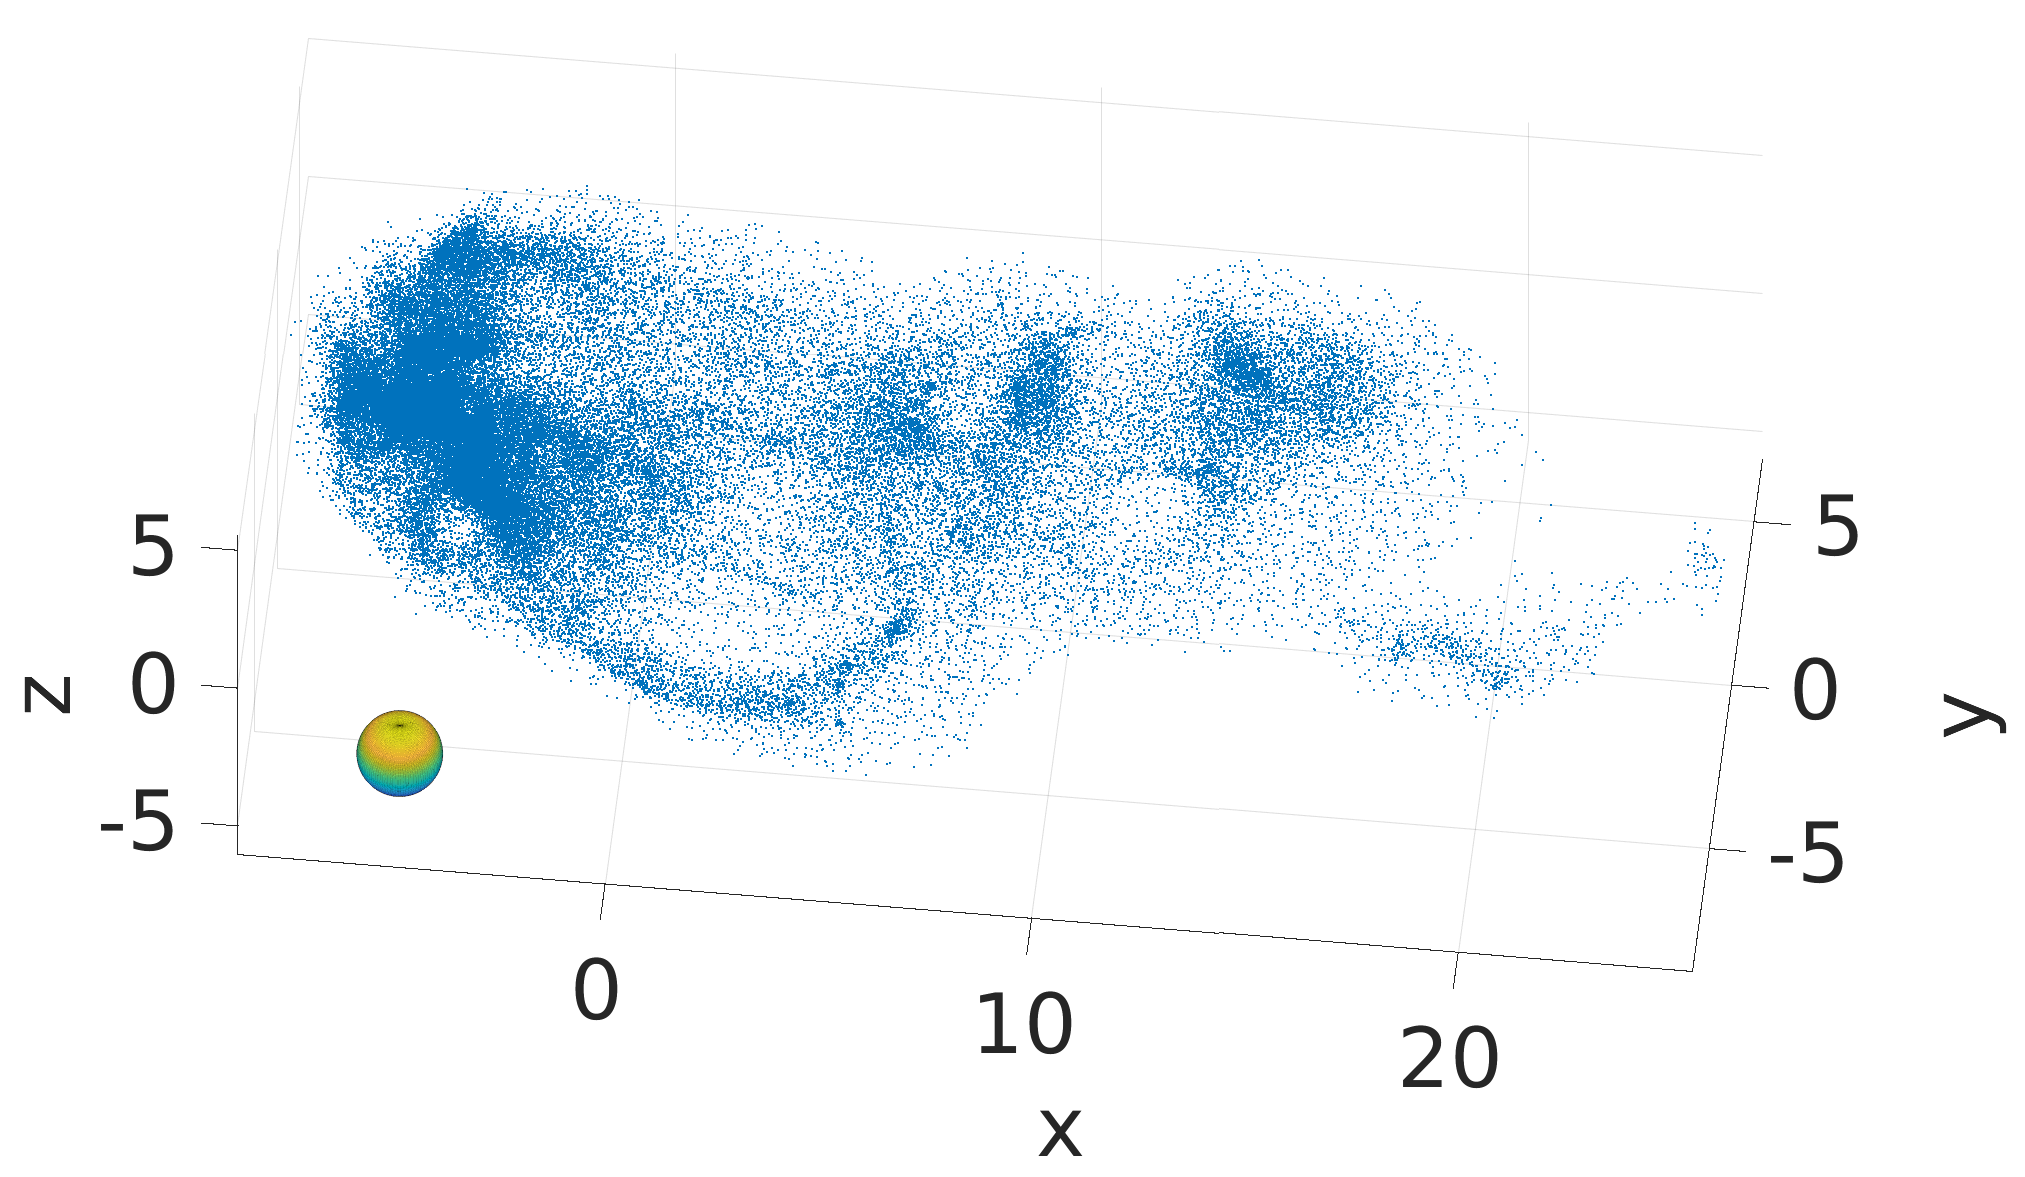
\includegraphics[width=\textwidth]{Figures_png/JF_Dataset}
    \caption{Gas particles having $\rho \ge 10^{-3} ~ \mathrm{atoms/cm^3}$ of the simulated dwarf galaxy falling into the halo of the Fornax Galaxy Cluster.}
    \label{fig:JF_Dataset}
\end{figure}
Starting from an existing suite of simulations of dwarf galaxies evolving in a Fornax-like cluster environment, we chose a single snapshot representing an irregular, gas rich galaxy, exposing an elongated star forming tail during intense ram pressure stripping. We want to investigate the geometry of their star forming regions.
% The simulation is performed using a modified version of the mixed N-body/Smoothed Particle Hydrodynamics (SPH) code GADGET-2 \cite{Springel2005, DeRijcke2013}. The simulation output consists of three types of particles: Dark Matter (DM), stellar and gaseous.
In particular, we will concentrate on morphology of gas with density $\rho \ge 10^{-3} ~ \mathrm{atoms/cm^3}$, % FIXME are we sure?
since this is a reasonable condition for it to be visible in the observed electromagnetic bandwidth.
\begin{figure}[ht]
    \centering
    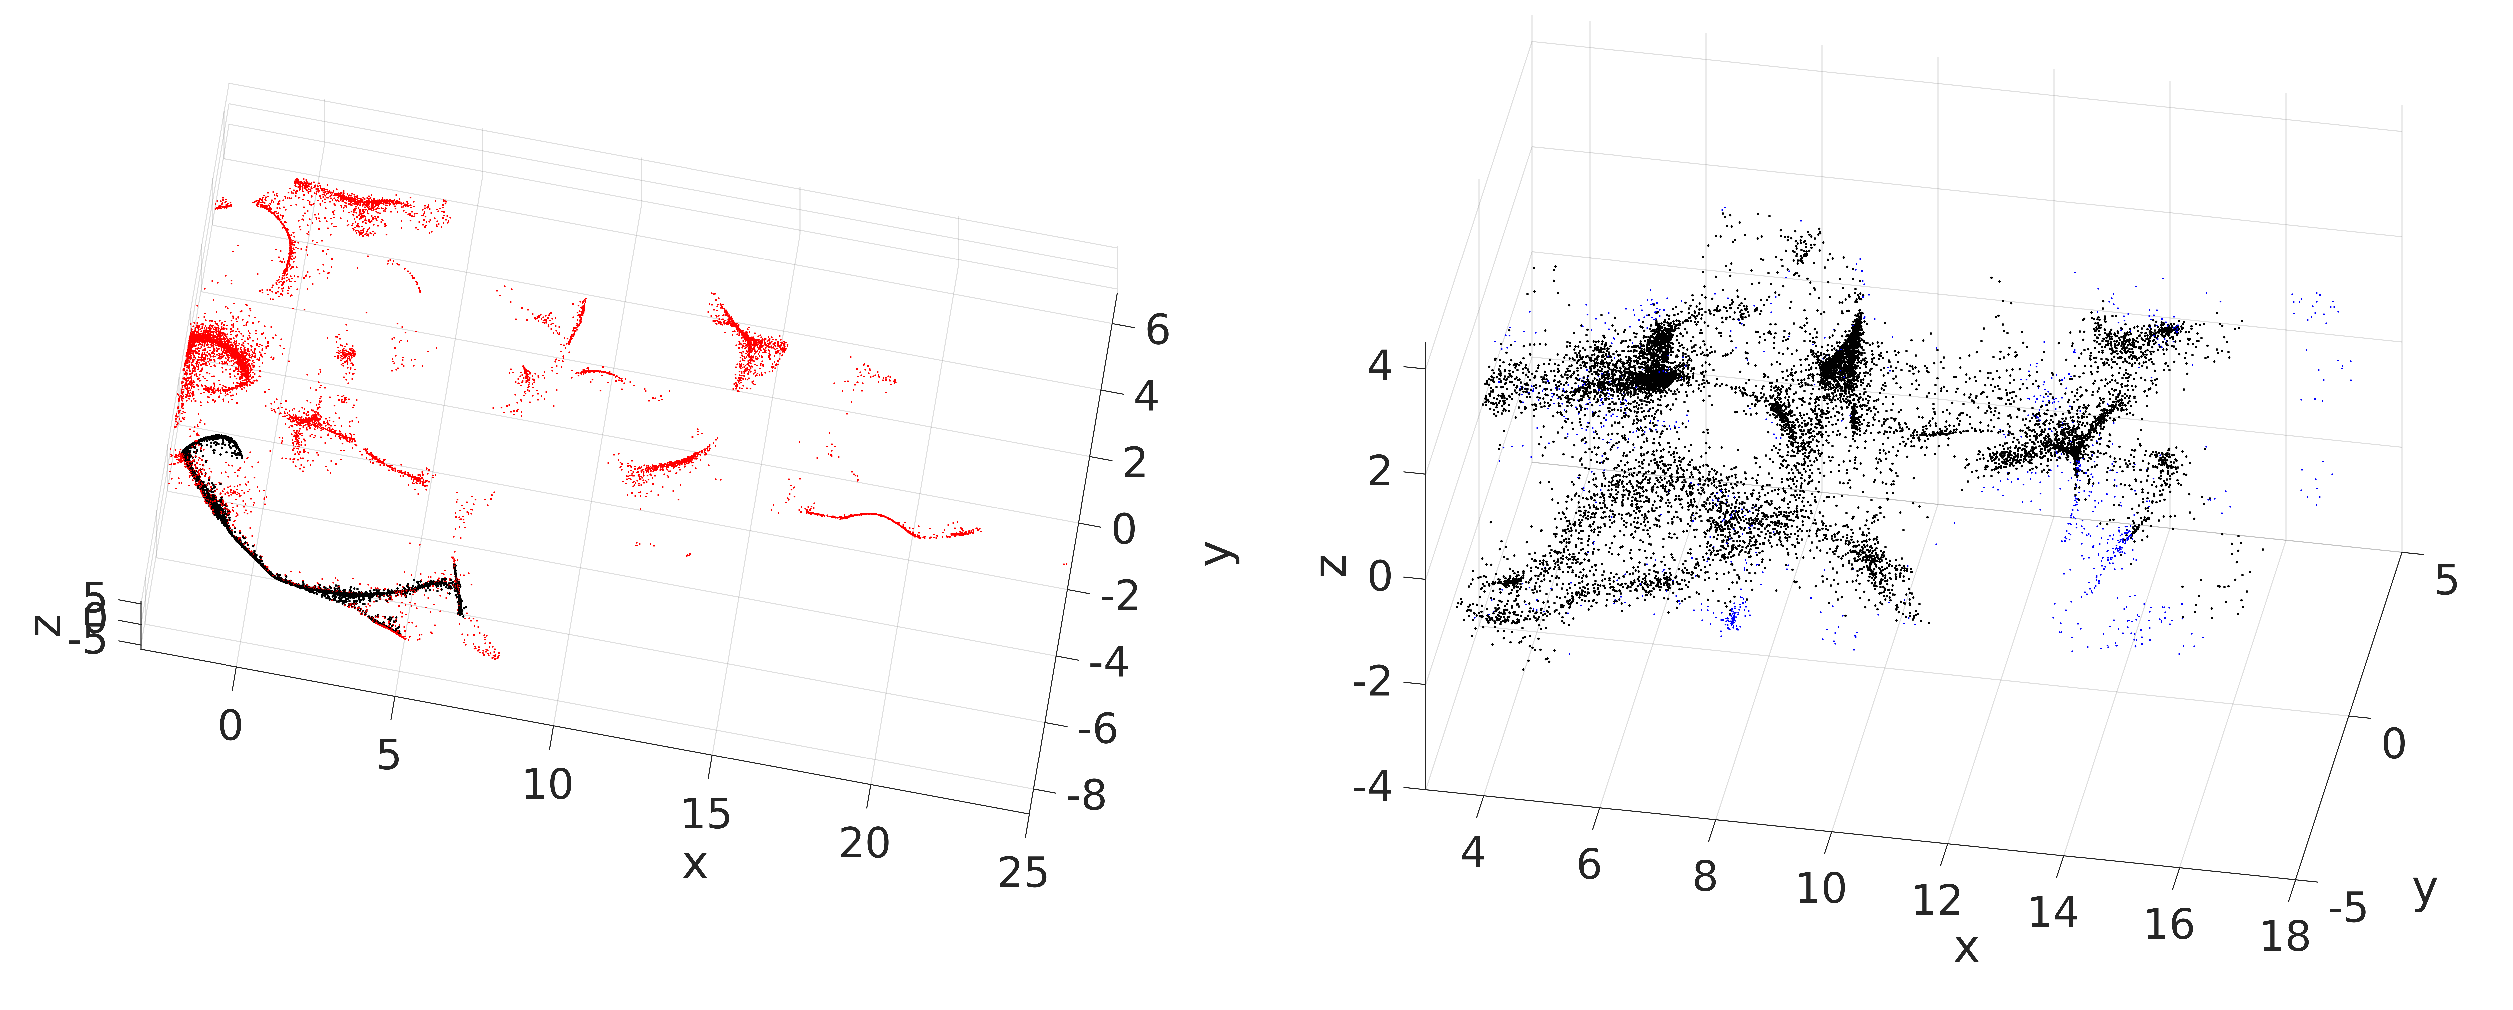
\includegraphics[width=\textwidth]{Figures_png/JF_SAF_Index_Man_v3}
    \caption{1-D (left) and 2-D (right) distributions of the diffused particles in the tail of the jellyfish structure.
    Highlighted in black are the points belonging to two distinct 1-D and 2-D structures discussed in section \ref{subsec:NGC1427A}.}
    \label{fig:JF_Res}
\end{figure}
We disregard DM and stellar particles (needed for evolution of the object, but not relevant for our analysis) and concentrate on the distribution of gas particles. The computation model is based on a particle formulation of hydrodynamics where each particle samples physical properties (mass, temperature, density etc.) of a volume of radius $r_N$ - radius of the sphere containing $N$ neighbouring particles. A continuous distribution of the physical variables over the full domain is then obtained by spatial smoothing with Gaussian kernels centered on each particle \cite{1977MNRAS.181..375G}. Associated with each gas particle (representing the corresponding volume) are values of  physical quantities such as density, temperature, pressure etc. Of particular interest is the intensity of the [CII] emission line. This is the "forbidden" line emitted by a carbon atom which has been ionized - having 5 out of 6 electrons. The outermost electron of the ionized atom gets excited on a higher energy level by radiation. The excited electron, under extremely low density environment conditions, is able to re-emit radiation at a specific wavelength ($158 ~ \mathrm{\mu m}$) while jumping to a lower energy level. These types of emission lines are called "forbidden" due to their impossibility to be seen in normal terrestrial environments.
They are, however, commonly observed in astronomy ([HII], O[III], etc.). Recent observations with the Herschel Space Observatory showed a tight correlation between the intensity of [CII] and other well known tracers of Star Formation Rate (SFR) \cite{DeLooze2011,Herrera_Camus_2015}. [CII] emission in this kind of simulations is obtained by using evolved quantities of the gas (metallicity, density and temperature) as inputs of chemical evolution models of the radiating gas, taking into account its ionization equilibrium and ion level occupation model \cite{Maio2007, DeRijcke2013}.

The resulting gas particle data set is presented in fig. \ref{fig:JF_Dataset}. Several low dimensional structures are clearly visible, for example the long 1-dimensional manifold departing from the head and elongating along the x-axis of the simulation box. Visually inspecting the data set, we chose a radius $r = 1 ~ \mathrm{kpc}$ as the characteristic scale parameter for the manifolds (shown as the small sphere in fig. \ref{fig:JF_Dataset}). This observation is reassuring, given that it is in agreement with the spatial resolution of recent observations. This parameter is fixed for preprocessing through diffusion and filtering (section \ref{sec:Method}), local dimensionality estimation (section \ref{subsec:D_Index}) and manifold crawling (sections \ref{subsec:Crawling} and \ref{subsec:MulitCrawl}).
% The other parameters are set as in the synthetic data experiments of section \ref{subsec:MulitCrawl}: $\epsilon=1$, $\eta=0.75$ and $\beta=0.4$.

As mentioned earlier, the main body of the data set can be visually divided into head and tail parts.
However, from the topological standpoint there is no justification for clear segregation into 1-D manifolds in the tail and 2-D manifolds in the head.
Dimensionality index estimation clearly identified 1-D structures in the tail, such as the elongated stream of particles starting from the head.
However, points in the head were also predominantly identified as 1-D, due to its complicated, intertwined filamentary structure.
On the other hand, distribution of 2-D points was more localized in the main body of the tail.


\section{A Multi Manifold analysis of a dwarf Jellyfish galaxy}\label{sec:manifold_jellyfish}

Having obtained the multi-manifold probabilistic profile of the gas particles in the tail of the jellyfish galaxy, 
it is possible to perform various kinds of detailed analysis of how physical properties vary along the manifolds.
Here we concentrate on the curvature (figure \ref{fig:curvatureJF}), as defined in section \ref{subsec:curvature} and on the star formation potential.
The latter is analysed by studying the the behaviour of emission line [CII] over the 1-D and 2-D structures
in the jellyfish tail shown as black dots in Figure~\ref{fig:JF_Res} (left) and (right), respectively
- the gaseous stream of gas particles departing from the head and reaching half way through the tail and the predominant 2-D structure in the tail.
\begin{figure}[ht]
\centering
\begin{subfigure}[t]{0.49\textwidth}
 \caption{}
 \label{subfig:CurvJF}
 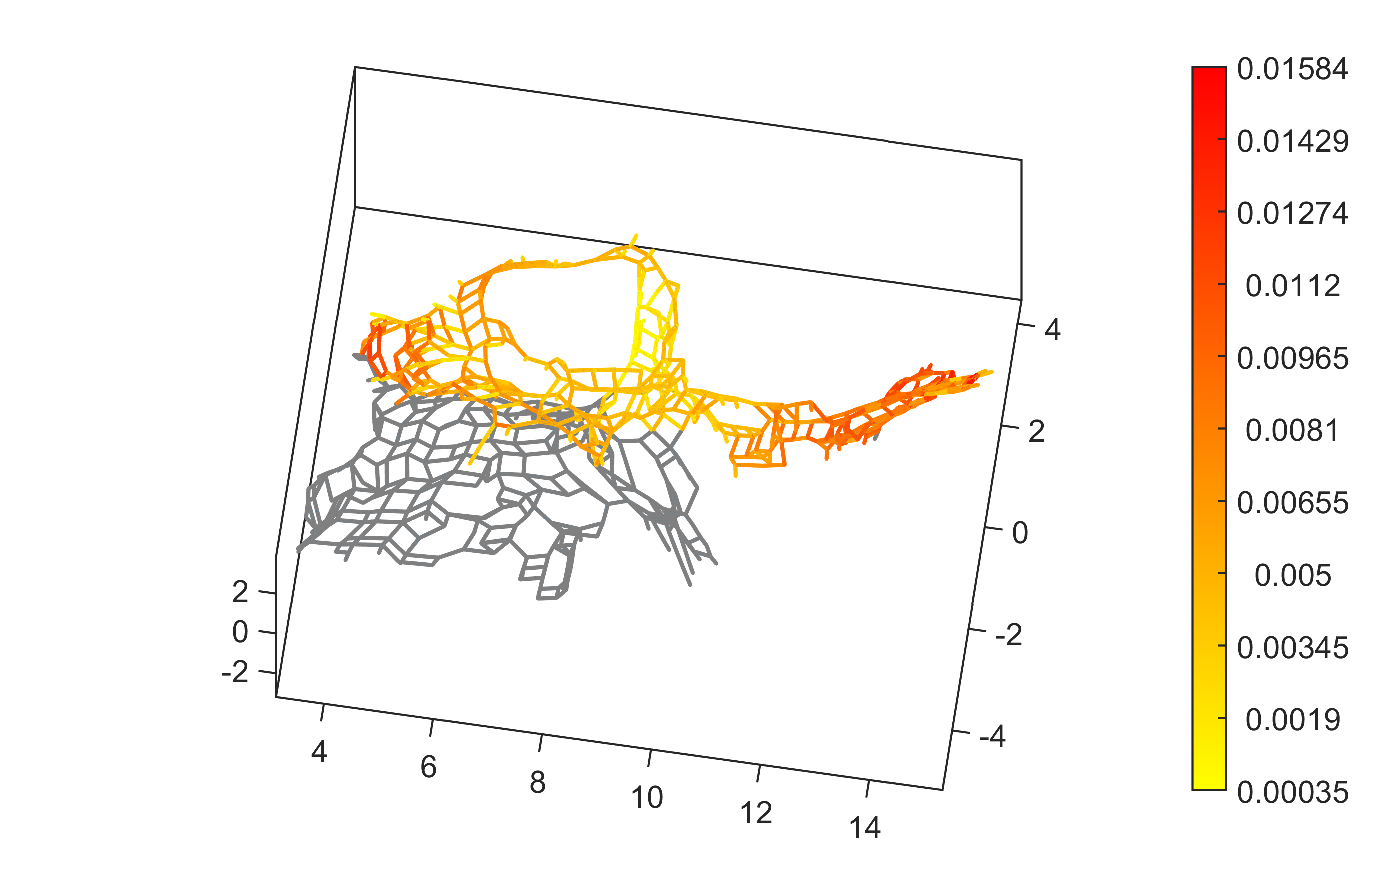
\includegraphics[width=\textwidth,trim = 100 0 150 0 ,clip = true]{Figures_png/Curvature_2DMan1_2.png}
\end{subfigure}
\begin{subfigure}[t]{0.49\textwidth}
 \caption{}
 \label{subfig:CurvJF_Plane}
 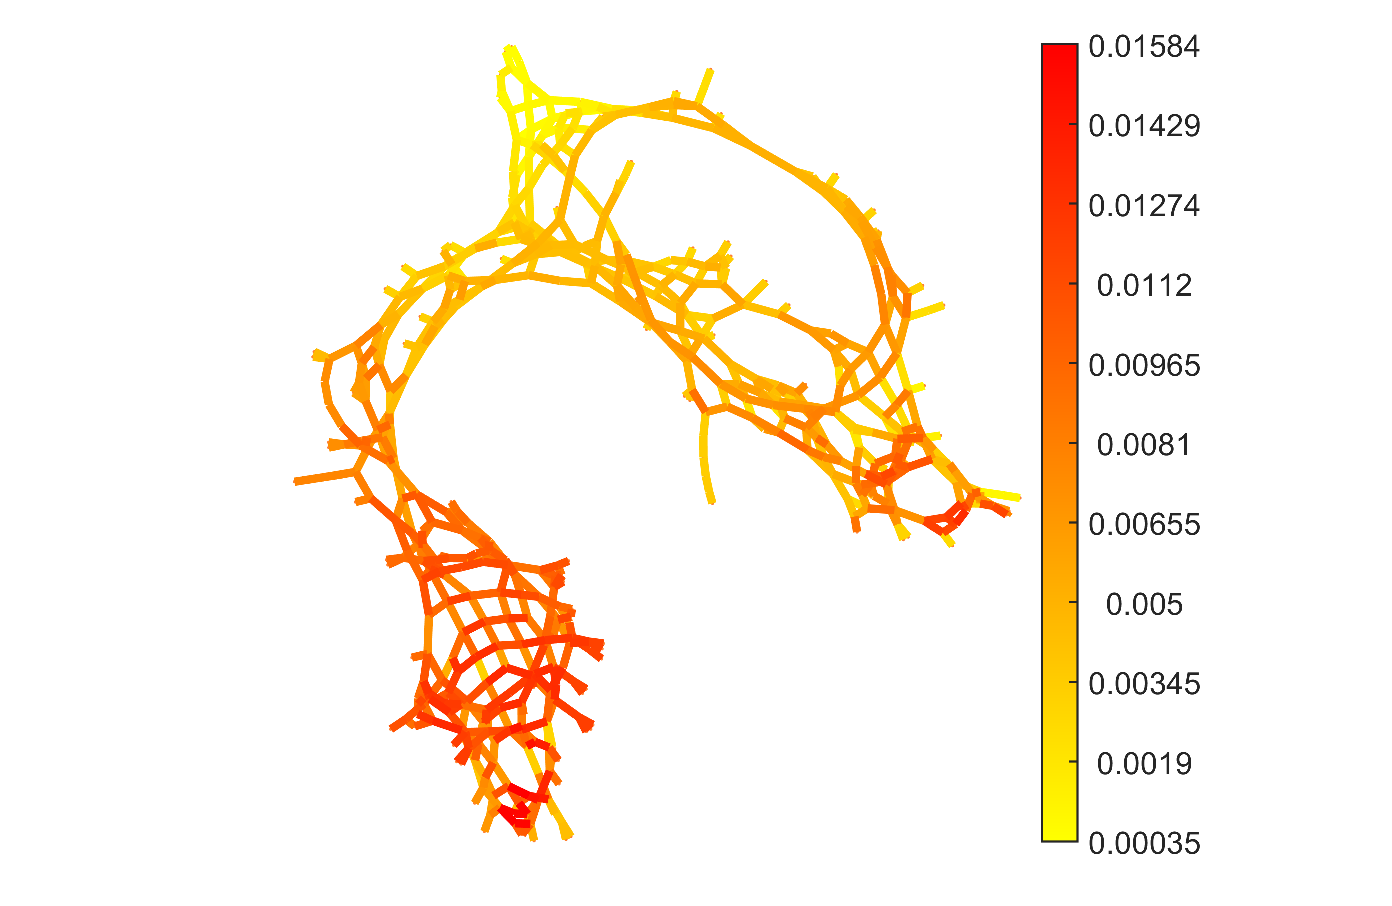
\includegraphics[width=\textwidth,trim = 50 0 75 0,clip=true]{Figures_png/Curvature_2DMan1_OnPlane.png}
\end{subfigure}
\caption{Embedded graph (a) and planar representation (b) of a 2-dimensional manifold extracted from the jellyfish data set, and its on-edge curvature distribution.}
\label{fig:curvatureJF}
\end{figure}

Figure \ref{subfig:CurvJF} shows two regions of high curvature, for the 2-dimensional manifold presented in figure \ref{fig:JF_Res}, right panel.
The far right region of intense curvature, is located towards the end of the tail, where the gas motion is more chaotic due to the motion of the galaxy through the halo of the galaxy cluster. However, the spherical region on the left side of the manifold, presenting a coherent curvature throughout its elongation (top right corner of figure \ref{subfig:CurvJF_Plane}) suggests, as a possible cause of formation, an isotropic expansion, typical of Supernova remnants. 

Taking advantage of the probabilistic nature of the AGTM model, we show in figure \ref{subfig:1dManGraph} the embedded vertices
$\bar{\vect{v}}_j$ of the graph $\bar{\cal G}$
for the stream model, with intensity modulated by the weighted mean of [CII] values $\mathcal{I}^{\mathrm{[CII]}}_i$ of particles $\vect{t}_i$ in the manifold, where the weights are the posterior probabilities of the node $v_j$, given  particles $\vect{t}_i$:
\begin{equation}\label{eq:WeightedVar}
    \overline{\mathcal{I}}^{\mathrm{[CII]}}_j = \frac{\sum_{i=1}^{N_{\mathcal{M}}} p(v_j | \vect{t}_i,\zeta_j\Sigma_j,\vect{W}_j) ~ \mathcal{I}^{\mathrm{[CII]}}_i}{\sum_{k=1}^{N_{\mathcal{M}}} p(v_j | \vect{t}_k,\zeta_j\Sigma_j,\vect{W}_j)}
\end{equation}
Analogous figure for the 2-D structure is presented in fig. \ref{subfig:2dManGraph}.

In the 1-D case, the manifold is located at the outskirts of the Jellyfish (fig. \ref{fig:JF_Dataset}, left panel), meaning that it is more exposed during the evolution to the surrounding gas of the galaxy cluster. This implies that the manifold is subject to a higher ram pressure than the tail, leading to a higher density and lower temperature of the gas - necessary conditions for the formation of new stars. These conditions are reflected in an increase of the [CII] emission line over the middle section of the manifold, $3 < x < 6$, thus informing us of an enhanced Star Formation Rate, compared to the rest of the manifold.
\begin{figure}[ht]
\centering
\begin{subfigure}[t]{0.48\textwidth}
 \caption{}
 \label{subfig:1dManGraph}
 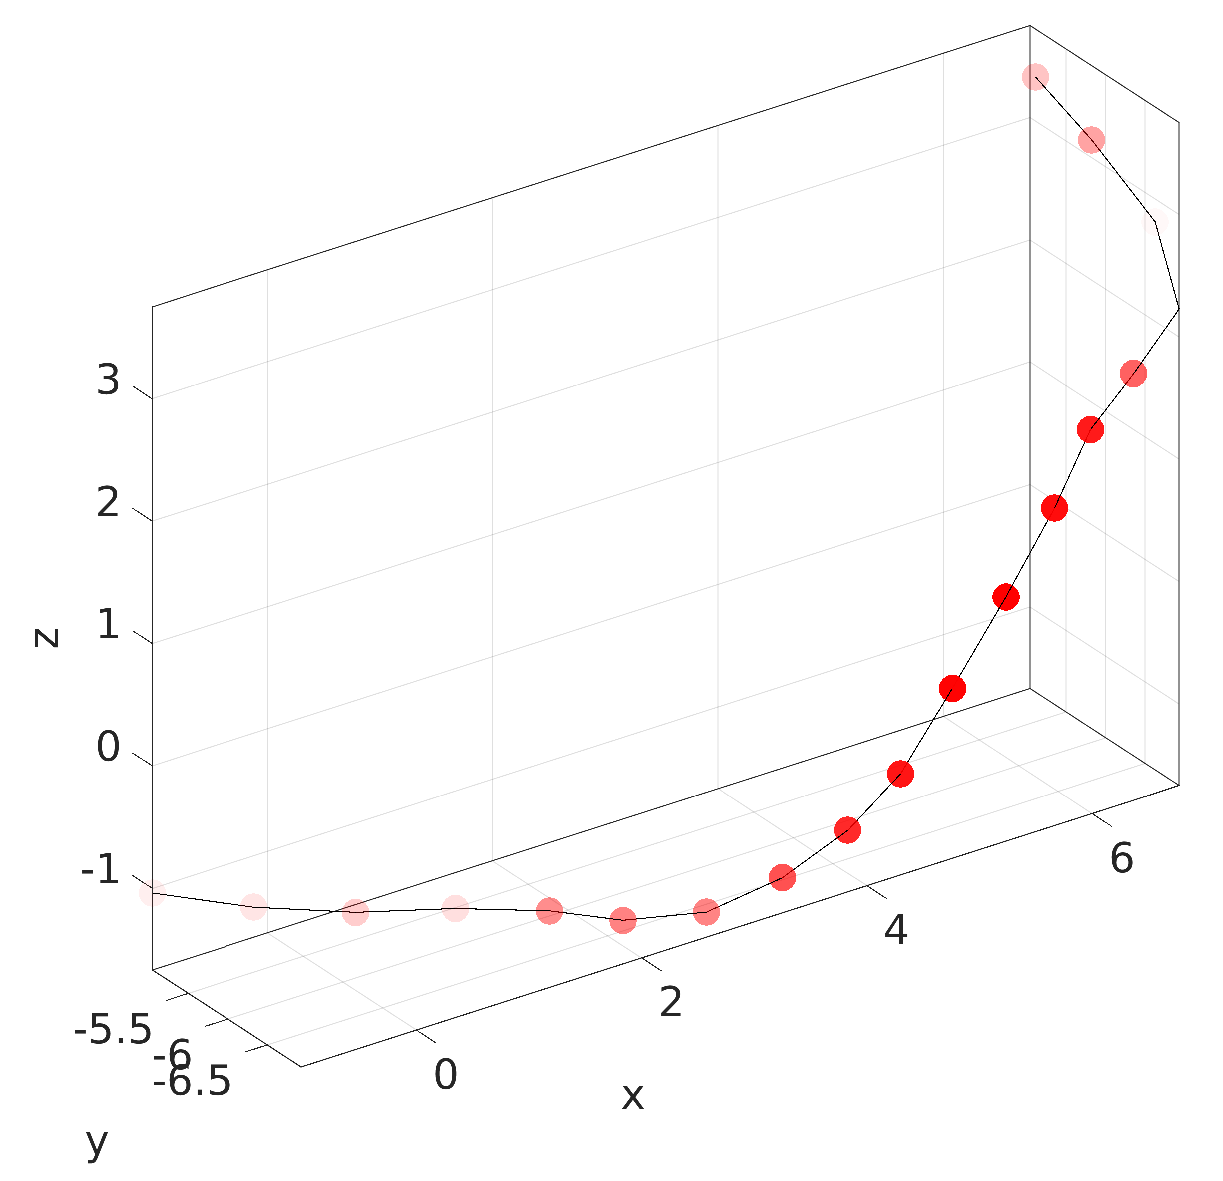
\includegraphics[width=\textwidth]{Figures_png/Manifold1D_AGTM2_cii_Shading}
\end{subfigure}
\begin{subfigure}[t]{0.49\textwidth}
 \caption{}
 \label{subfig:2dManGraph}
 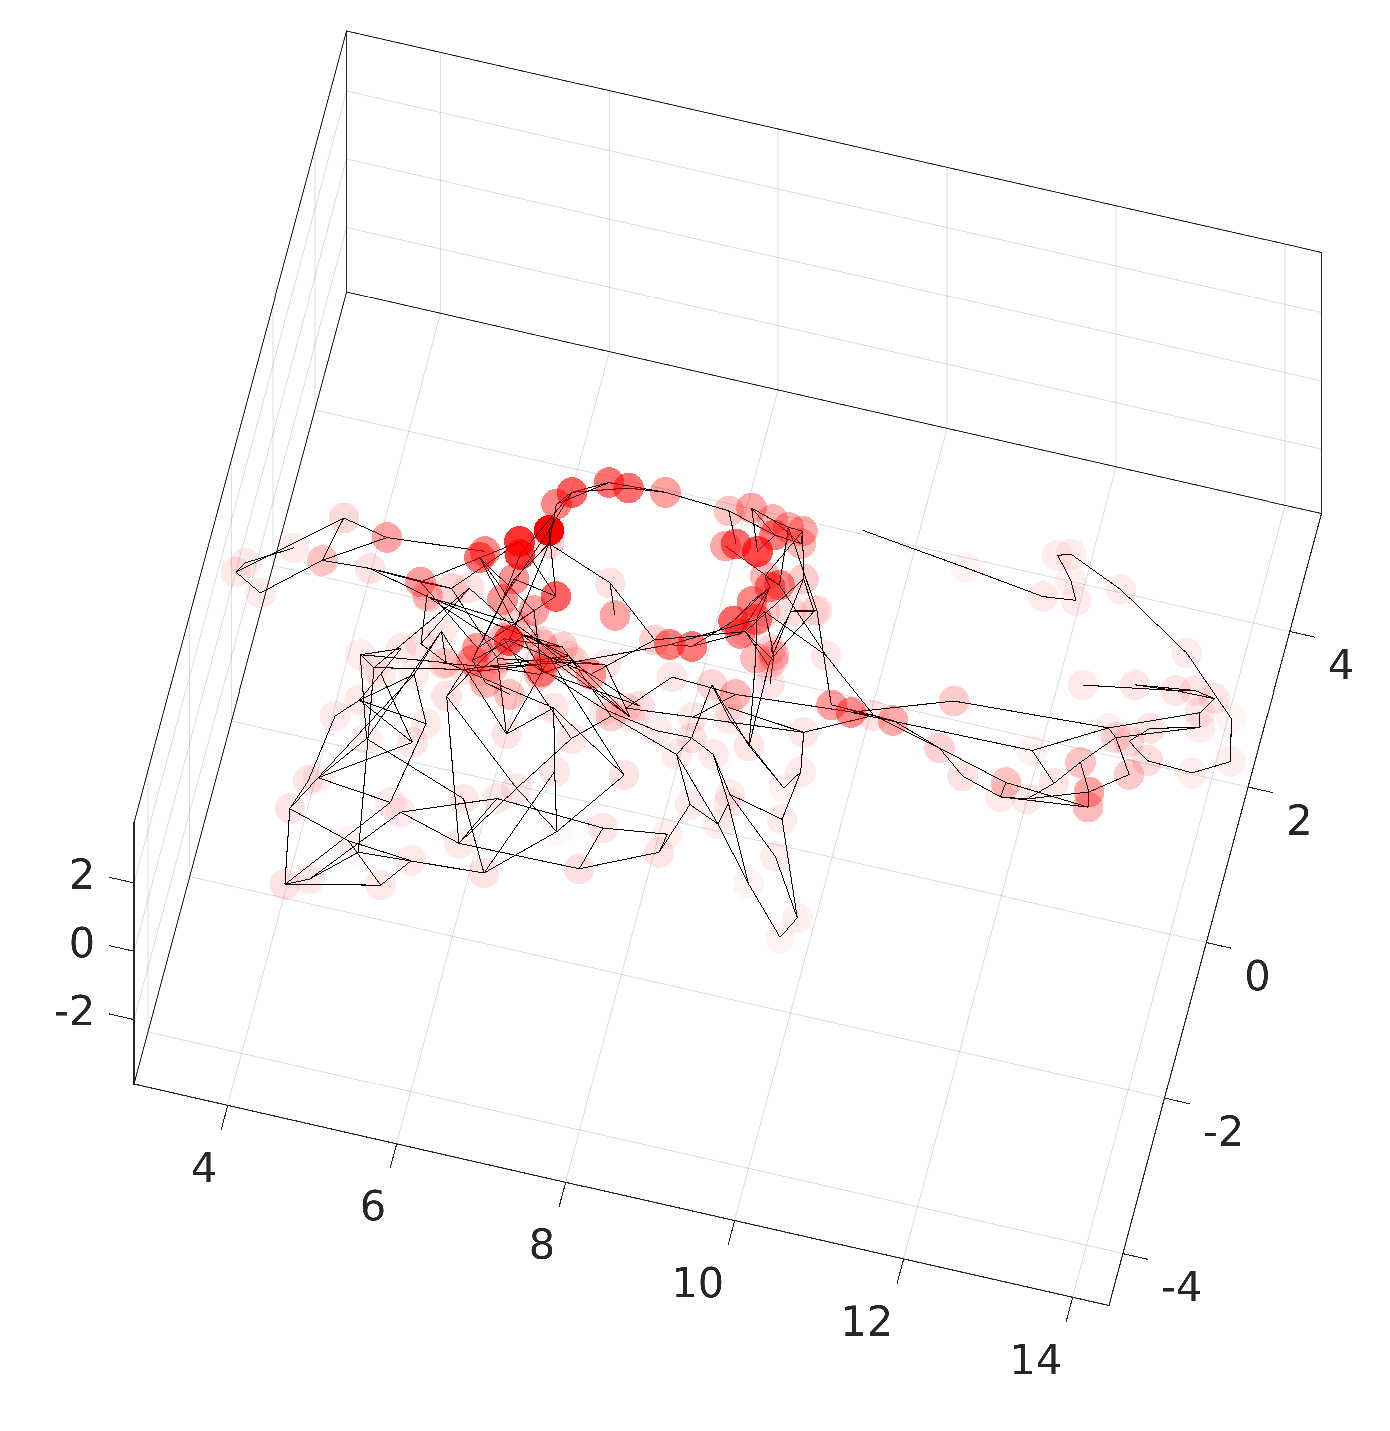
\includegraphics[width=\textwidth]{Figures_png/Manifold2D_AGTM2_cii_Shading}
\end{subfigure}
\caption{1D (a) and 2D (b) manifolds extracted from the data set in Figure~\ref{fig:JF_Dataset}.
The graphs' nodes are colored based on the value of [CII] of the surrounding particles lying not further than $\mathrm{1~kpc}$ from the local tangent space of the manifold, weighted by the nodes' responsibilities.}
\label{fig:Man2D}
\end{figure}

The 2-D structure shows an overall constant [CII] intensity whereas the region at $5 < x < 9$ presents sharply higher values.
The shape of this region is particularly interesting. It is, in fact, a hole with an almost spherical section. This structure detected with AGTM and Manifold Crawling, with potent [CII] emission at its boundary, is the remnant of a supernova explosion. Due to their high mass, young stars burn efficiently and relatively fast all their gas reservoir, terminating their life as supernovae and injecting energy and debris in the surroundings.
This process is modeled in the simulation via an injection of $10^{51}$~erg of energy for a short amount of time and a transfer of metallic elements (in the case of our simulation, the model tracks iron and magnesium, \cite{DeRijcke2013}) to the neighbouring gas particles. The metal-enriched gas particles (like in the surrounding of a supernova explosion) are then able to cool down more efficiently and show strong [CII] emission line. 

Our methodology provides a strong tool for extracting such an information from the morphology of gas particles and can be used to effectively calibrate feedback models \footnote{By feedback mechanisms, we mean any process that allows to exchange energy, matter and/or momentum among galaxy components.} in simulations.

Such a detailed analysis of low dimensional structures (remnants of galaxy interactions) is not currently possible with tools routinely used to calibrate and analyse astrophysical simulations of galaxy evolution.
As mentioned in section \ref{subsec:MulitCrawl}, the technique presented in this paper can be used as a semi-automatic exploratory tool by the domain experts, where the focus and characteristic scale of the structures to be mined can be varied continuously with analysis of their physical properties of interest (after necessary computations) performed and studied on the fly.
